\ifdefined\handout
  \documentclass[handout]{beamer}
\else
  \documentclass{beamer}
\fi

\usetheme{boxes}
\usecolortheme{structure}

\setbeamertemplate{footline}[frame number]

\ifdefined\handout
\definecolor{beamer@structure@color}{rgb}{0,0,0}
\setbeamertemplate{navigation symbols}{}
\setbeamercolor{normal text}{fg=black,bg=white}
\setbeamertemplate{frametitle}{\vskip 15pt\color{black}
\def\myhrulefill{\leavevmode\leaders\hrule height 1pt\hfill\kern 0pt}
\headingfont\insertframetitle\par\vskip-8pt\myhrulefill}
\else
\definecolor{beamer@structure@color}{rgb}{1,1,1}
\setbeamertemplate{navigation symbols}{}
\setbeamercolor{normal text}{fg=white,bg=black}
\setbeamertemplate{frametitle}{\vskip 15pt\color{white}
\def\myhrulefill{\leavevmode\leaders\hrule height 1pt\hfill\kern 0pt}
\headingfont\insertframetitle\par\vskip-8pt\myhrulefill}
\fi

\usepackage{amsmath,amssymb}

\newcommand{\NN}{\mathbb{N}}
\newcommand{\ZZ}{\mathbb{Z}}

\DeclareMathOperator{\mcd}{mcd}
\DeclareMathOperator{\mcm}{mcm}

\usepackage[spanish]{babel}

\usepackage{tikz-cd}
\usetikzlibrary{babel}
\usetikzlibrary{calc}

\usepackage{framed}

\newcommand{\dfn}{\mathrel{\mathop:}=}
\newcommand{\rdfn}{=\mathrel{\mathop:}}

\usepackage{mathspec}
\setsansfont[BoldFont={IBM Plex Sans Bold}, ItalicFont={IBM Plex Sans Italic}]{IBM Plex Sans}
\setmonofont[BoldFont={IBM Plex Mono Bold}, ItalicFont={IBM Plex Mono Italic}]{IBM Plex Mono}
\setmathrm[BoldFont={IBM Plex Sans Bold}, ItalicFont={IBM Plex Sans Italic}]{IBM Plex Sans}
\newfontfamily\headingfont[]{IBM Plex Sans Bold}

\setbeamercovered{transparent=10}


\usepackage{multicol}
\setlength{\columnseprule}{1pt}

\tikzset{xcenter around/.style 2 args={execute at end picture={%
  \useasboundingbox let \p0 = (current bounding box.south west), \p1 = (current bounding box.north east),
                        \p2 = (#1), \p3 = (#2)
                    in
        ({min(\x2 + \x3 - \x1,\x0)},\y0) rectangle ({max(\x3 + \x2 - \x0,\x1)},\y1);
}}}

\begin{document}

\begin{frame}[plain,noframenumbering]
  \textbf{INTRODUCCIÓN A LA TEORÍA DE NÚMEROS}

  Alexey Beshenov $\mid$ \texttt{cadadr.org}

  \vfill

  \begin{center}\huge\headingfont
    LEMAS DE GAUSS Y EUCLIDES
  \end{center}

  \vfill
\end{frame}

\begin{frame}
  \frametitle{MOTIVACIÓN}

  \begin{itemize}
  \item<2-> \textbf{Teorema fundamental de la aritmética}: para $a > 0$
    $$a = p_1 \cdots p_s,$$
    donde los $p_i$ son primos, \underline{definidos de modo único}, salvo permutación.

  \item<3-> Resultado no tan obvio.

    Primera prueba rigurosa: Gauss.

  \item<4-> Hoy: lema de Gauss y lema de Euclides.
  \end{itemize}
\end{frame}

\begin{frame}
  \frametitle{LEMA DE GAUSS}

  \begin{minipage}[t][0.6\textheight]{0.6\textwidth}
    \vspace{0pt}
    \onslide<2->{Si $\mcd (d,a) = 1$ y $d \mid ab$, \\
      entonces $d \mid b$.}

    \vspace{1em}

    \onslide<3->{\textbf{Demostración}.}

    \onslide<4->{\[ d \mid \mcd (db, ab) = b\cdot \mcd (d,a) = b. \qed \]}
  \end{minipage}
  \begin{minipage}[t]{0.35\textwidth}
    \vspace{0pt}\flushright
    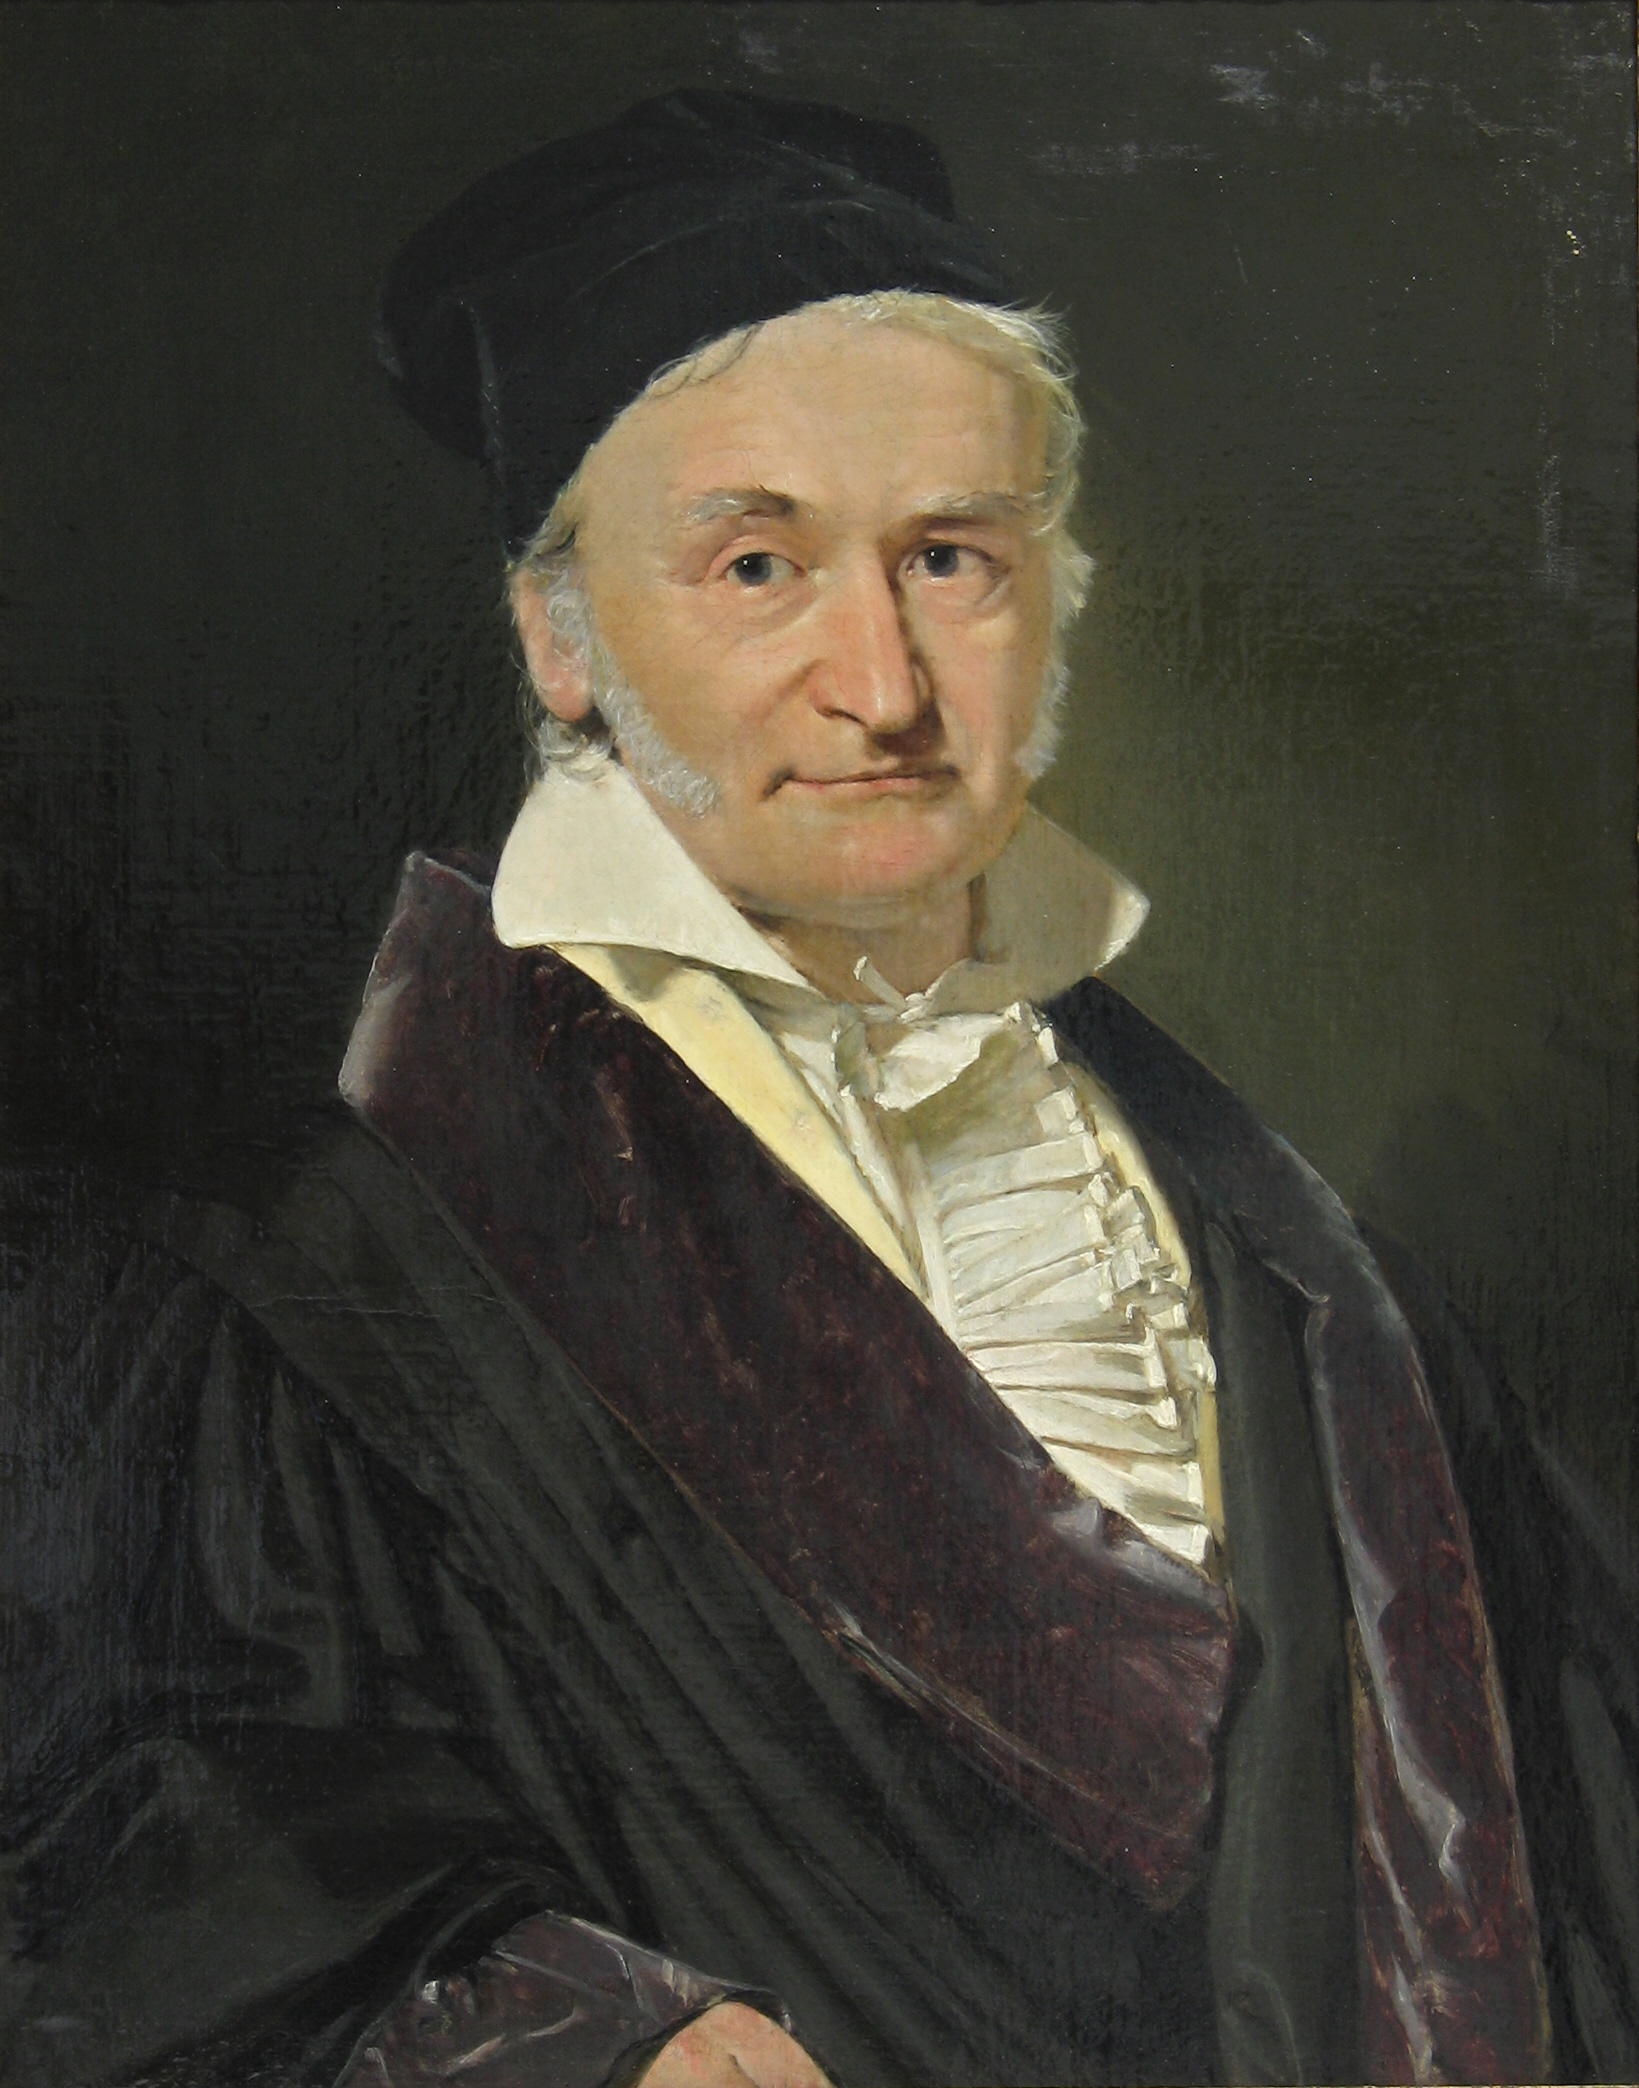
\includegraphics[width=.9\textwidth]{gauss.jpg}

    Carl Friedrich Gauß \\
    (1777--1855)
  \end{minipage}
\end{frame}

\begin{frame}
  \frametitle{APLICACIÓN: REPRESENTACIÓN ÚNICA DE LOS NÚMEROS RACIONALES}

  \onslide<2->{\begin{framed}
      Cada número racional $x \ne 0$ se representa de modo único como
      \[ x = \frac{a}{b}, \quad a > 0, ~ \mcd (a,b) = 1. \]
    \end{framed}}

  \onslide<3->{\textbf{Demostración}.}

  \begin{gather*}
    \onslide<4->{\frac{a}{b} = \frac{a'}{b'}, ~ a, a' > 0, ~ \mcd (a,b) = \mcd (a',b') = 1.} \\
    \onslide<5->{a \mid ab' = a'b, ~ \mcd (a,b) = 1}
    \onslide<6->{\Longrightarrow a \mid a',} \\
    \onslide<7->{a' \mid a'b = ab', ~ \mcd (a',b') = 1}
    \onslide<8->{\Longrightarrow a' \mid a,} \\
    \onslide<9->{a = a',} \quad \onslide<10->{b = b'. \qed}
  \end{gather*}
\end{frame}

\begin{frame}
  \frametitle{EJERCICIO}

  \onslide<2->{\begin{framed}
      Si $\mcd (a,b) = \mcd (c,d) = 1$ y
      \[ \frac{a}{b} + \frac{c}{d} \in \ZZ, \]
      entonces $b = \pm d$.
    \end{framed}}
\end{frame}

\begin{frame}
  \frametitle{APLICACIÓN: IRRACIONALIDAD DE $\sqrt{2}$}

  \onslide<2->{\begin{framed}
      El número
      \[ \sqrt{2} = 1.41421356237309504880\ldots \]
      es irracional: no existe un número racional $x = \frac{a}{b}$ tal que
      $x^2 = 2$.
    \end{framed}}

  \onslide<3->{\textbf{Demostración}.}

  \onslide<4->{Sea $x = \frac{a}{b}$ con $\mcd (a,b) = 1$.}

  \begin{gather*}
    \onslide<5->{x^2 = 2 \iff a^2 = 2b^2.} \\
    \onslide<6->{\mcd(a,b) = 1, ~ b \mid a^2 \Longrightarrow b \mid a.}
  \end{gather*}

  \onslide<7->{Contradicción. \qed}
\end{frame}

\begin{frame}
  \frametitle{LOS PITAGÓRICOS Y LA IRRACIONALIDAD}

  La irracionalidad de $\sqrt{2}$ fue descubierta por los pitagóricos y guardada
  como un secreto.

  \begin{center}
    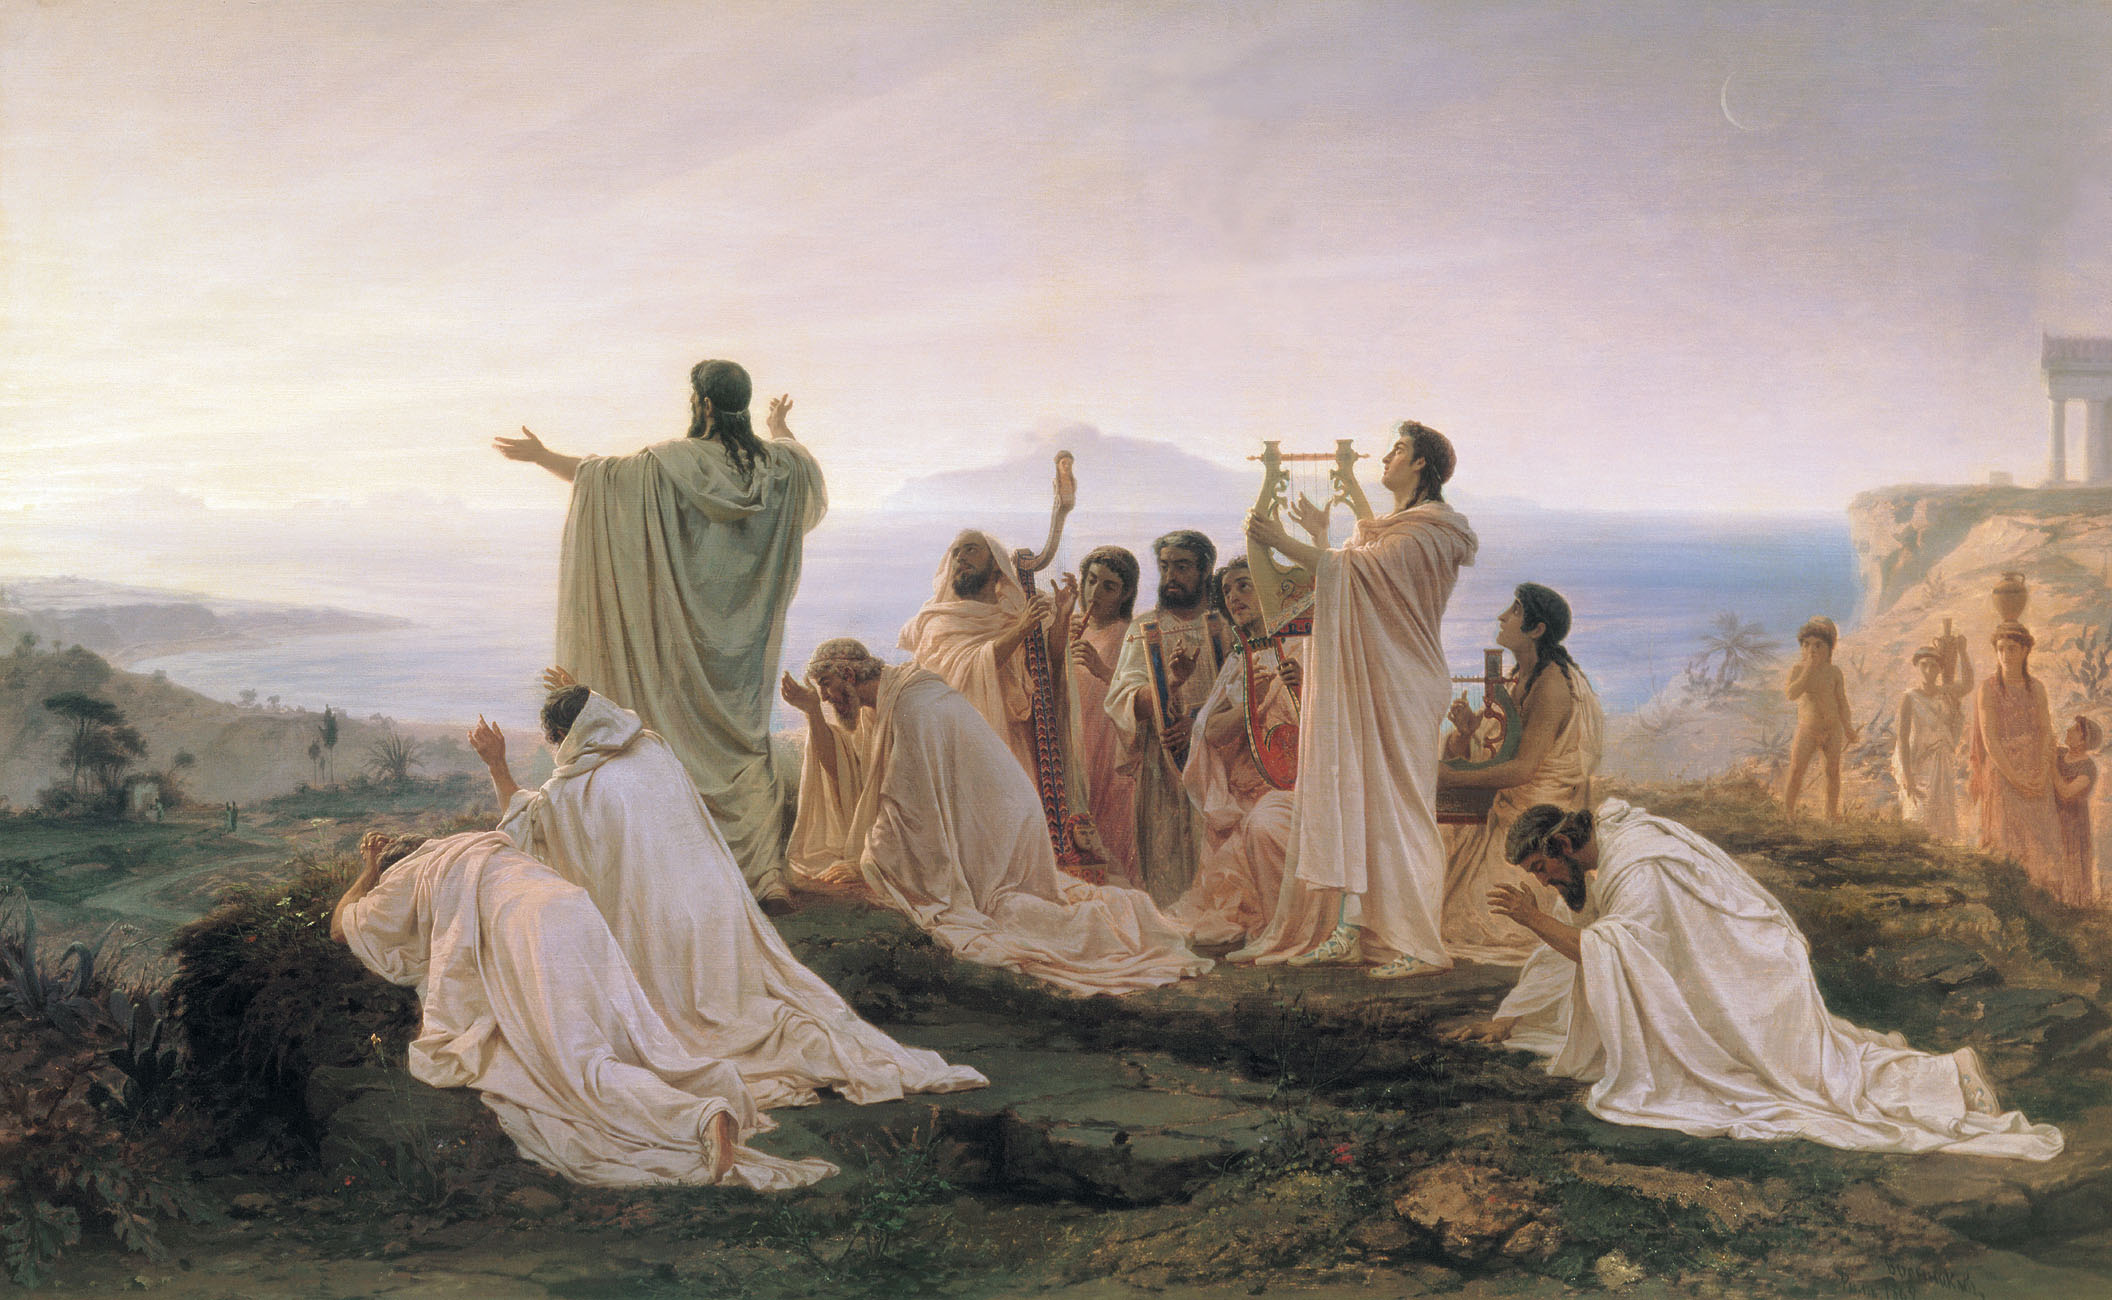
\includegraphics[width=0.8\textwidth]{pitagoricos.jpg}

    Pitagóricos celebrando la salida del sol. \\
    Fyodor Bronnikov, 1869
  \end{center}
\end{frame}

\begin{frame}
  \begin{center}
    \begin{tikzpicture}[x=5cm,y=5cm,xcenter around={0.5,0.5}{0.5,0.5}]
      \draw (0,0) edge node[below] {$1$} (1,0);
      \draw (1,0) edge node[right] {$1$} (1,1);

      \draw (1,1) -- (0,1);
      \draw (0,1) -- (0,0);

      \draw (0,0) edge node[above left] {$\sqrt{2}$} (1,1);
    \end{tikzpicture}

    \vspace{1em}

    La diagonal es \textbf{inconmensurable}\\
    con respecto a los lados
  \end{center}
\end{frame}

\begin{frame}
  \frametitle{HÍPASO DE METAPONTO}

  \begin{minipage}[t][0.6\textheight]{0.6\textwidth}
    \vspace{0pt}
    \begin{itemize}
    \item<2-> Según algunas fuentes,

      Hípaso de Metaponto reveló al mundo la
      existencia de los números irracionales.

    \item<3-> ¿Murió en un naufragio en circunstancias misteriosas?

    \item<4-> ¿Se suicidó como autocastigo?

    \item<5-> ¿Fue arrojado al mar por los pitagóricos?
    \end{itemize}

  \end{minipage}
  \begin{minipage}[t]{0.35\textwidth}
    \vspace{0pt}\flushright
        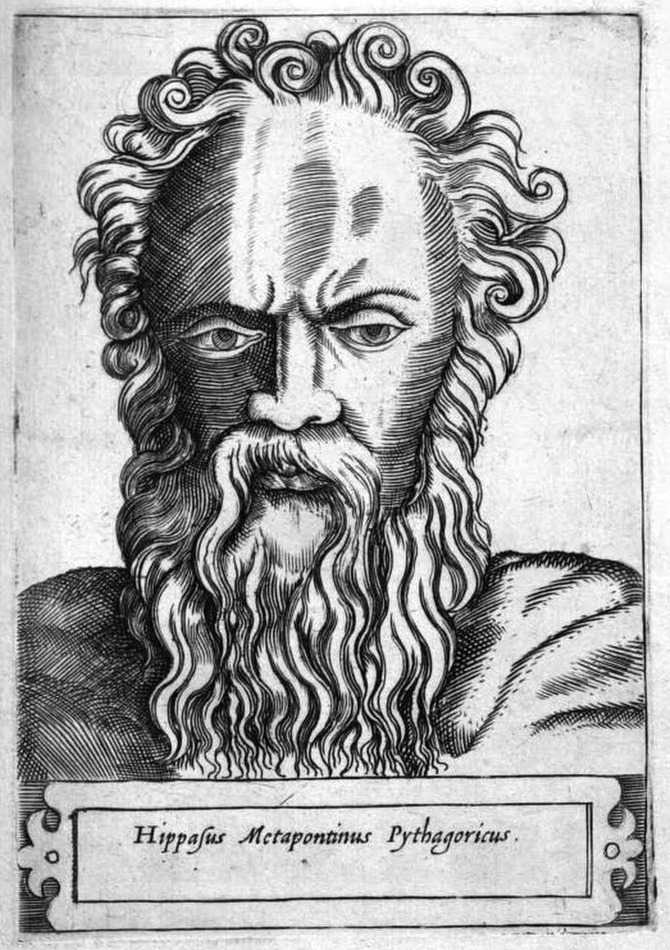
\includegraphics[width=.9\textwidth]{hipaso.jpg}

        Hípaso de Metaponto\\
        (ca. 530--450 a.C.)
  \end{minipage}
\end{frame}

\begin{frame}
  \frametitle{EJERCICIOS}

  \begin{itemize}
  \item<2-> Demuestre que $\sqrt[n]{a}$ es irracional si $a \in \ZZ$ no es la
    $n$-ésima potencia de algún entero.

  \item<3-> Demuestre que $\sqrt{2} + \sqrt{3}$ es irracional.

  \item<4-> ¡No se arroje al mar!
  \end{itemize}
\end{frame}

\begin{frame}
  \frametitle{LEMA DE EUCLIDES}

  \onslide<2->{\begin{framed}
      Para $p > 1$ las siguientes condiciones son equivalentes:
      \begin{enumerate}
      \item[a)]<3-> $p$ es primo; es decir, los únicos divisores positivos
        $d \mid p$ son $1$ y $p$;

      \item[b)]<4-> para cualesquiera $a, b \in \ZZ$, si $p \mid ab$, entonces
        $p \mid a$ o $p \mid b$.
      \end{enumerate}
    \end{framed}}

  \onslide<5->{\textbf{Demostración}.}

  \onslide<6->{a) $\Rightarrow$ b): lema de Gauss.}

  \onslide<7->{b) $\Rightarrow$ a):}
  \onslide<8->{\[ d \mid p \iff p = ad \Longrightarrow p \mid a\text{ o }p \mid d. \]}

  \onslide<9->{Si $p \mid a$, entonces $d = 1$.}

  \onslide<10->{Si $p \mid d$, entonces $d = p$. \qed}
\end{frame}

\begin{frame}
  \frametitle{EJERCICIO}

  \onslide<2->{\begin{framed}
      Si $p$ es primo y
      \[ p \mid a_1\cdots a_s, \]
      entonces $p\mid a_i$ para algún $i = 1,\ldots s$.
    \end{framed}}
\end{frame}

\begin{frame}
  \frametitle{«DISQUISITIONES ARITHMETICAE»}


  \begin{minipage}[t][0.6\textheight]{0.6\textwidth}
    \vspace{0pt}
    \begin{itemize}
    \item<2-> «Investigaciones aritméticas».

    \item<3-> Tratado de la teoría de números escrito por Gauss en 1798
      a la edad de 21 años.

    \item<4-> Primera publicación en 1801.

    \item<5-> Sistematización del trabajo prévio de
      Fermat, Euler, Lagrange, Legendre.

    \item<6-> Pruebas rigurosas de resultados fundamentales, incluyendo
      el teorema fundamental de la aritmética.

    \item<7-> Muchos resultados nuevos.
    \end{itemize}
  \end{minipage}
  \begin{minipage}[t]{0.35\textwidth}
    \vspace{0pt}\flushright
    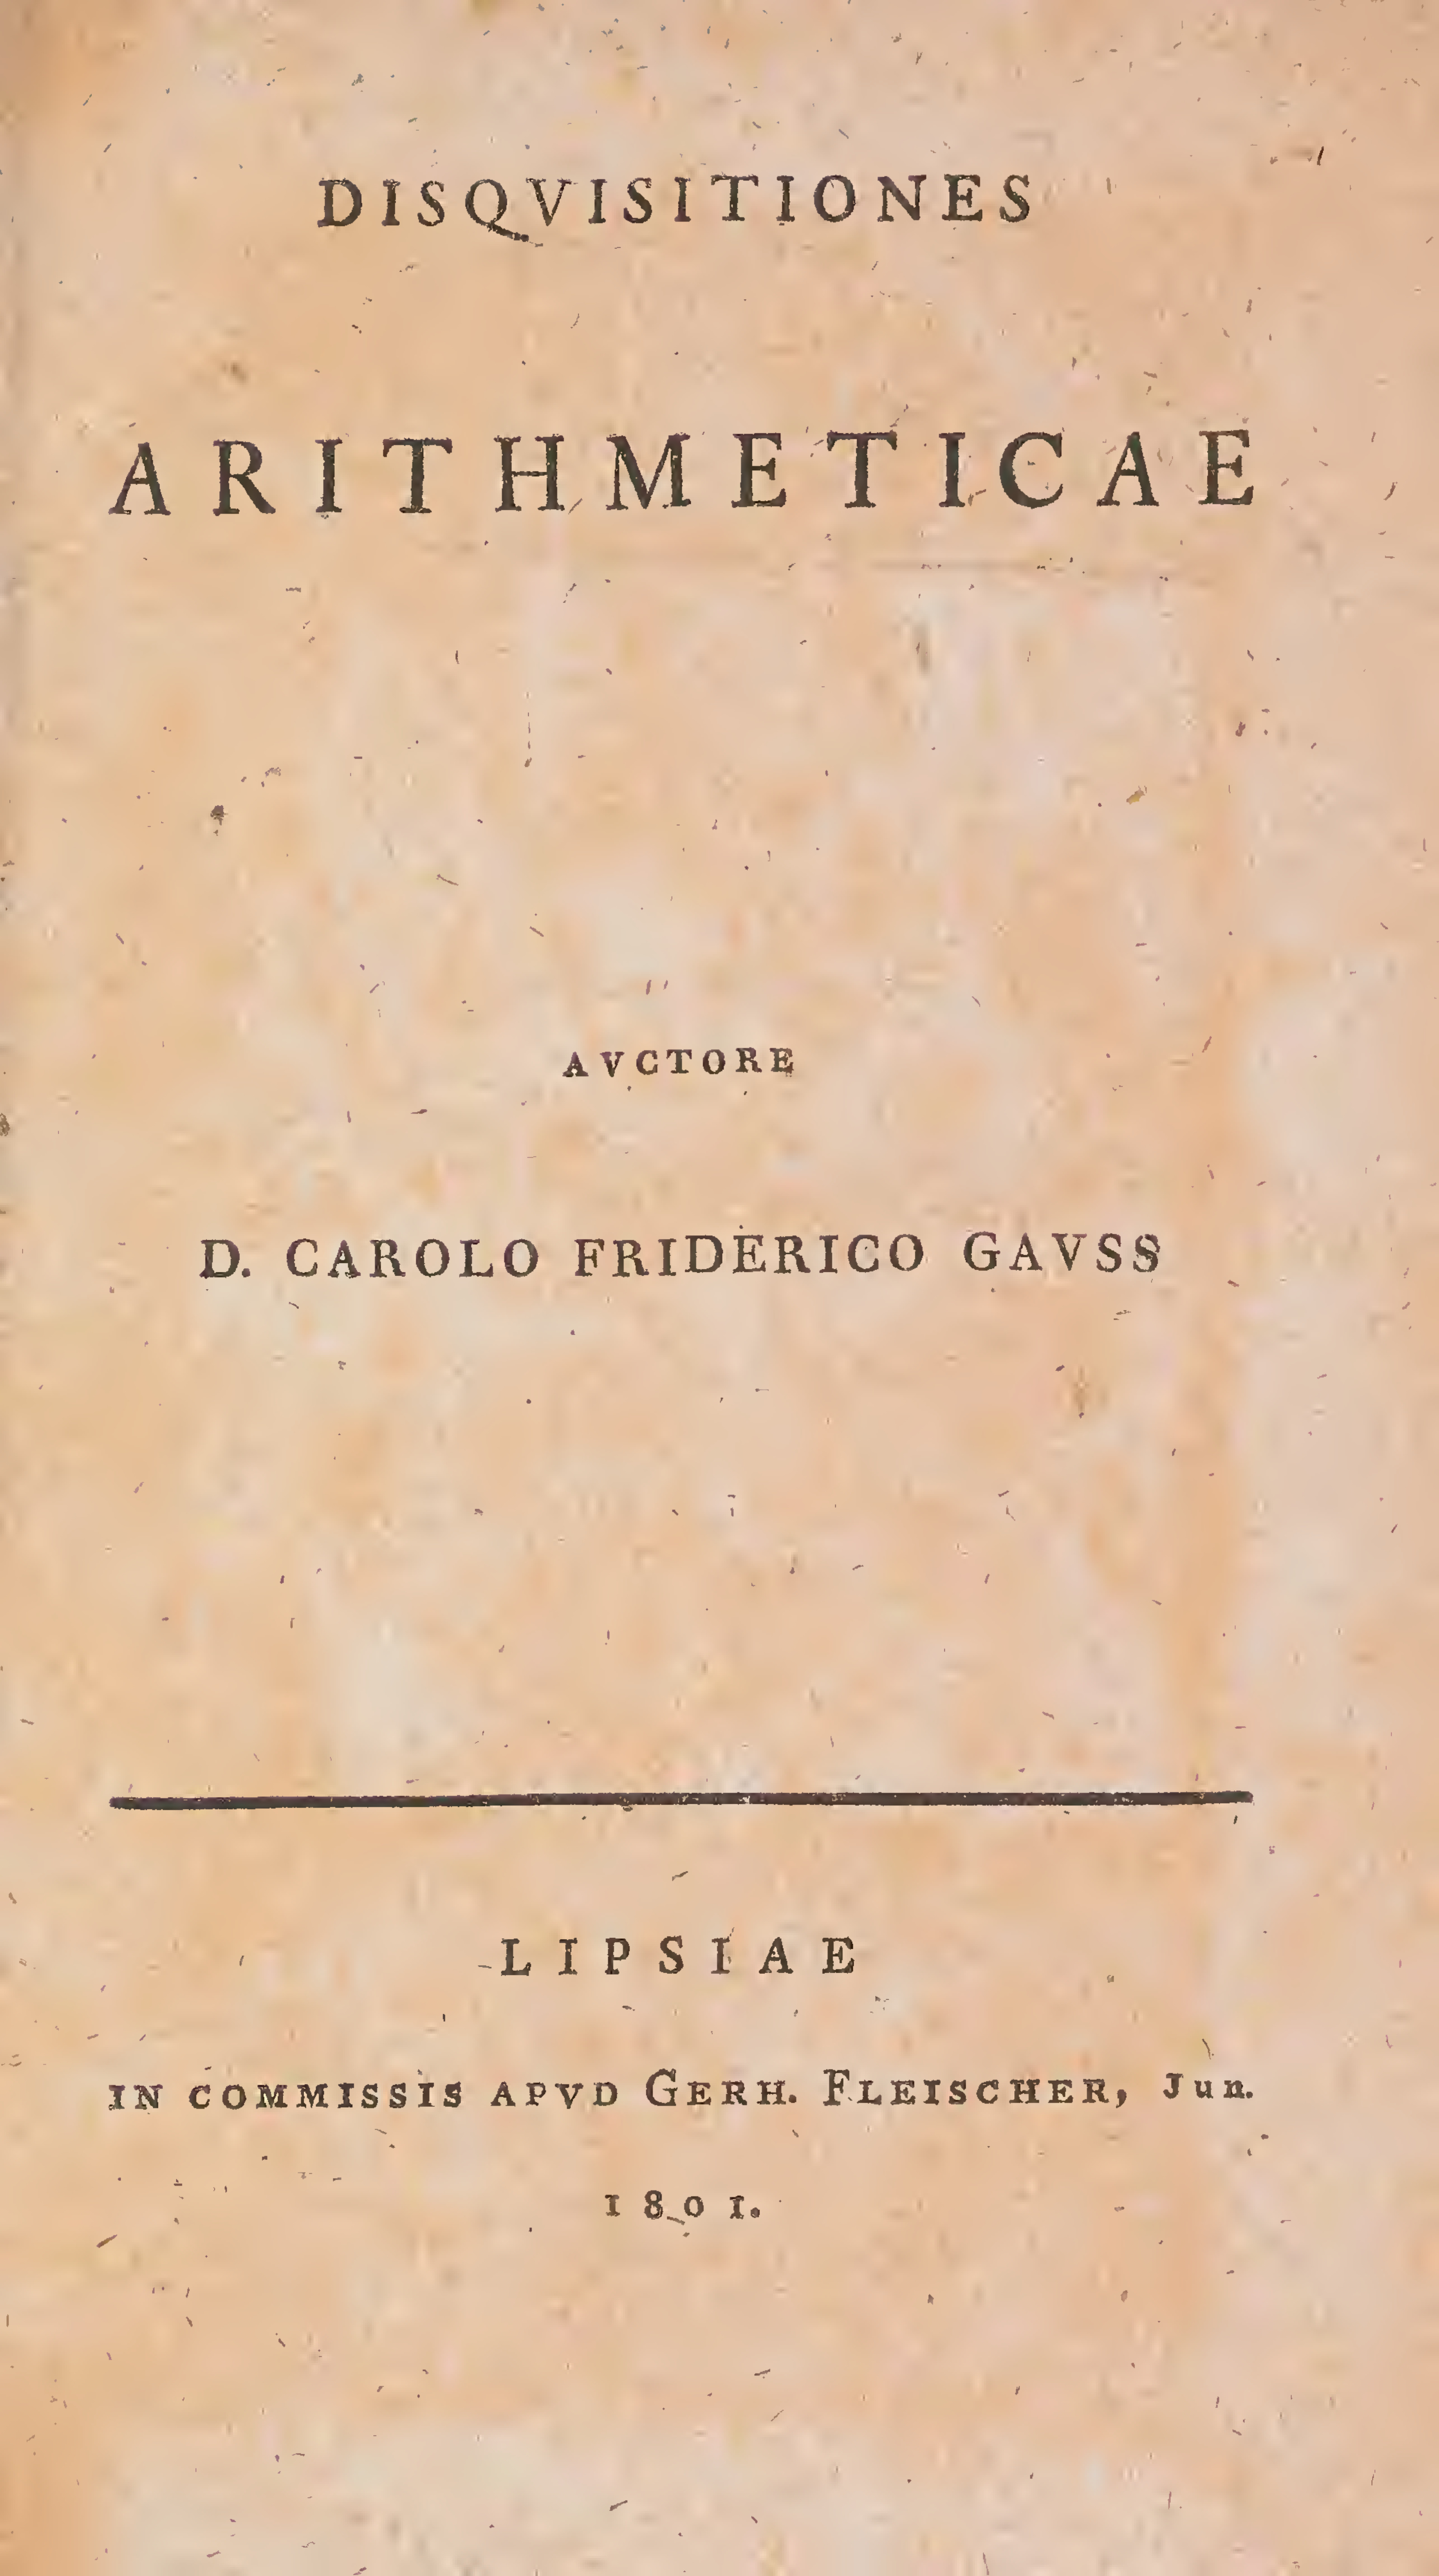
\includegraphics[width=.9\textwidth]{disquisitiones.jpg}
  \end{minipage}
\end{frame}

\begin{frame}
  \frametitle{«DISQUISITIONES», SECTIO SECUNDA, \S 14}

  \begin{center}
    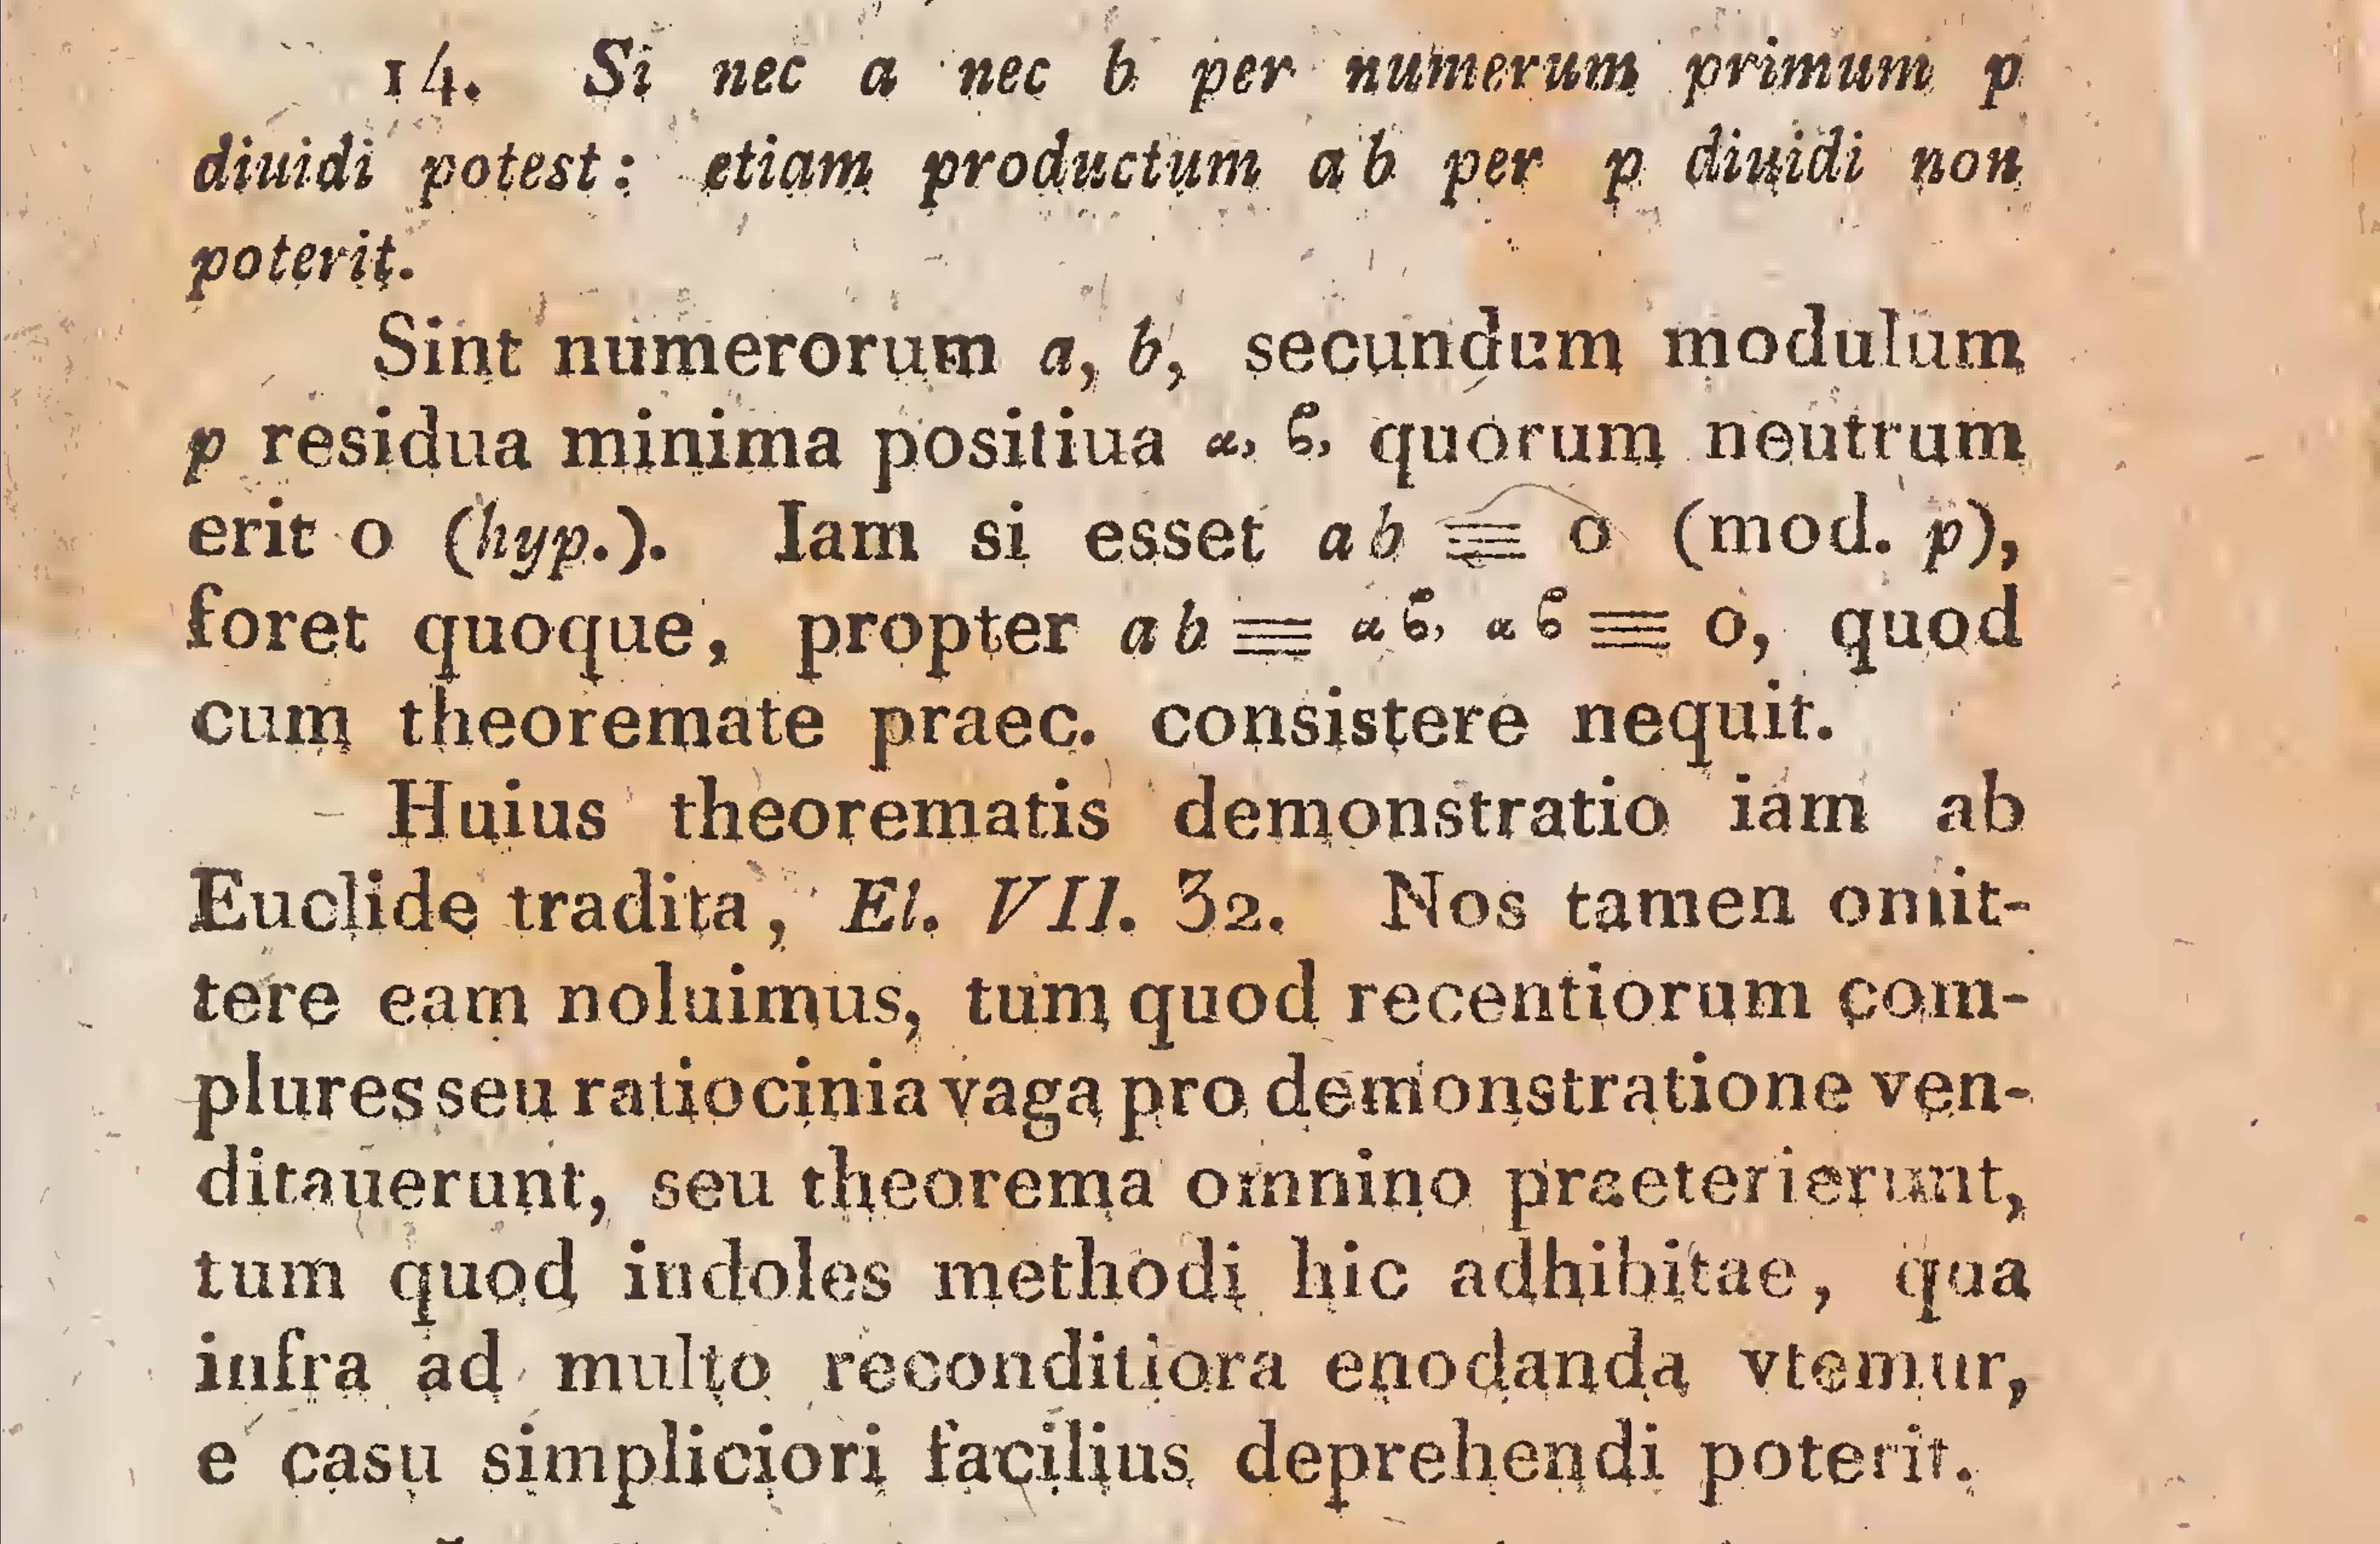
\includegraphics[width=.9\textwidth]{disquisitiones-14.jpg}

    «Si ni $a$ ni $b$ pueden dividirse por un número primo $p$, tampoco el
    producto $ab$ puede dividirse por $p$.»
  \end{center}
\end{frame}

\begin{frame}

  \begin{multicols}{2}\small
    Huius theorematis demonstratio iam ab Euclide tradita,
    \emph{El. VII. 32}. Nos tamen omittere eam noluimus, tum quod recentiorum
    complures seu ratio cinia vaga pro demonstratione venditauerunt,
    seu theorema omnio praeterierunt\dots

    \vfill\null
    \columnbreak

    Euclides ya había demostrado este teorema en sus «Elementos» (libro VII,
    no. 32). No obstante deseábamos no omitirlo puesto que muchos autores
    modernos han usado razonamientos inciertos en vez de demostraciones, o bien
    han despreciado el teorema completamente.
  \end{multicols}

  \texttt{centroedumatematica.com/aruiz/libros/\\
    DisquisitionesArithmeticae/}
\end{frame}

\begin{frame}[plain,noframenumbering]

  \vfill

  \begin{center}\huge\headingfont
    ¡GRACIAS POR SU ATENCIÓN!
  \end{center}

  \vfill
\end{frame}
\end{document}
